\subsection{Continuous Integration and Deployment (CI/CD)}
%olivia
%A complete description of stages and tools included in the CI/CD chains, including deployment and release of your systems.
%create a diagram!
To automate building, testing and releasing our ITU-MiniTwit system, we implemented a CI/CD pipeline using GitHub Actions. We chose GitHub Actions due to its native integration with our GitHub-hosted repository, ease of configuration, and support for open-source projects. This allowed us to set up an effective pipeline without maintaining external CI infrastructure, which aligned well with the size and scope of our team project.

\subsubsection*{Pipeline Overview}

Our pipeline is triggered on every push to the \texttt{main} branch and consists of three main stages: \textbf{build}, \textbf{test}, and \textbf{deploy}.

\begin{enumerate}
\item
\subsubsection*{Build Stage}
\begin{itemize}
  \item The pipeline checks out the code and logs into Docker Hub using secrets stored securely in GitHub.
  \item It then builds two Docker images:
    \begin{itemize}
      \item \texttt{devoops-app} (the frontend)
      \item \texttt{devoops-api} (the backend)
    \end{itemize}
  \item These images are tagged and pushed to Docker Hub, using cache layers for efficiency.
\end{itemize}

\item
\subsubsection*{Test Stage}
\begin{itemize}
  \item After successful builds, the pipeline spins up a full test stack using 
  \texttt{docker-compose\_test\_local.yml} which runs containerized tests.
  \item This includes integration, API, UI, and end-to-end tests. The pipeline will fail fast if any test fails, stopping the deployment stage to ensure only verified code is released.
\end{itemize}

\item
\subsubsection*{Deploy Stage}
\begin{itemize}
  \item This stage involves deploying to our remote infrastructure on DigitalOcean using a \texttt{blue-green deployment strategy} based on two floating IPs. The full upgrade logic and IP switching process is described separately in the Upgrade Strategy section.
  \item A step using \texttt{terraform init} is also executed to set up the infrastructure. While this ensures the environment is up-to-date, we acknowledge that re-running \texttt{terraform init} and \texttt{apply} on every push may be excessive and could be optimized to only run when infrastructure-related files change.
\end{itemize}
\end{enumerate}

\subsubsection*{Static Analysis \& Quality Gates}

We integrated multiple static analysis tools as quality gates into a pipeline that runs when a pull request is created, to catch code issues early and enforce consistent formatting and linting:
\begin{itemize}
  \item \texttt{gofmt} checks Go code formatting.
  \item \texttt{golangci-lint} performs static analysis on Go files.
  \item \texttt{dockerfilelint} validates all Dockerfiles.
\end{itemize}

\subsubsection*{Release Automation}

We automated our release process using a GitHub Actions workflow that triggers on tags matching \texttt{v*}, creating versioned GitHub Releases with auto-generated notes. This ensures consistent, traceable production releases aligned with our deployment flow.

\subsection{Monitoring}
\label{sec:monitoring}
We use Prometheus and Grafana to monitor our system’s health. Metrics are instrumented with the Prometheus Go client library, registered via the default Prometheus registry, and exposed through the \textit{metrics} endpoint for Prometheus to scrape. \\ \\ 
For visualization we use Grafana, that uses prometheus as a data source and enables us to create and customize panels that visualizes the different metrics. \\\\ 
In relation to the James Turnbull monitoring maturity model\cite{turnbull2015monitoring}, ours would be considered reactive as we track specific errors in relation to specific endpoints and overall availability.\\\\
We do not do any front-end monitoring, as the course was primarily focused on the simulations interaction with our API.
\subsubsection{Metrics monitored}
We defined the following endpoints. Some, like \textit{Successful requests} track multiple endpoints and aggregate them in single time line for easier viewing and a reduction in overall panels in Grafana. The full dashboard can be seen in figure \ref{fig:dashboard}
\begin{itemize}
    \item \textbf{Uptime}
    \item \textbf{Successful requests (Tracks multiple endpoints)}
    \item \textbf{Unsuccessful requests (Tracks multiple endpoints)}
    \item \textbf{Follows}
    \item \textbf{Unfollows}
    \item \textbf{Successful messages sent}
    \item \textbf{Users not found}
\end{itemize}

\begin{figure} [!htb]
    \centering
    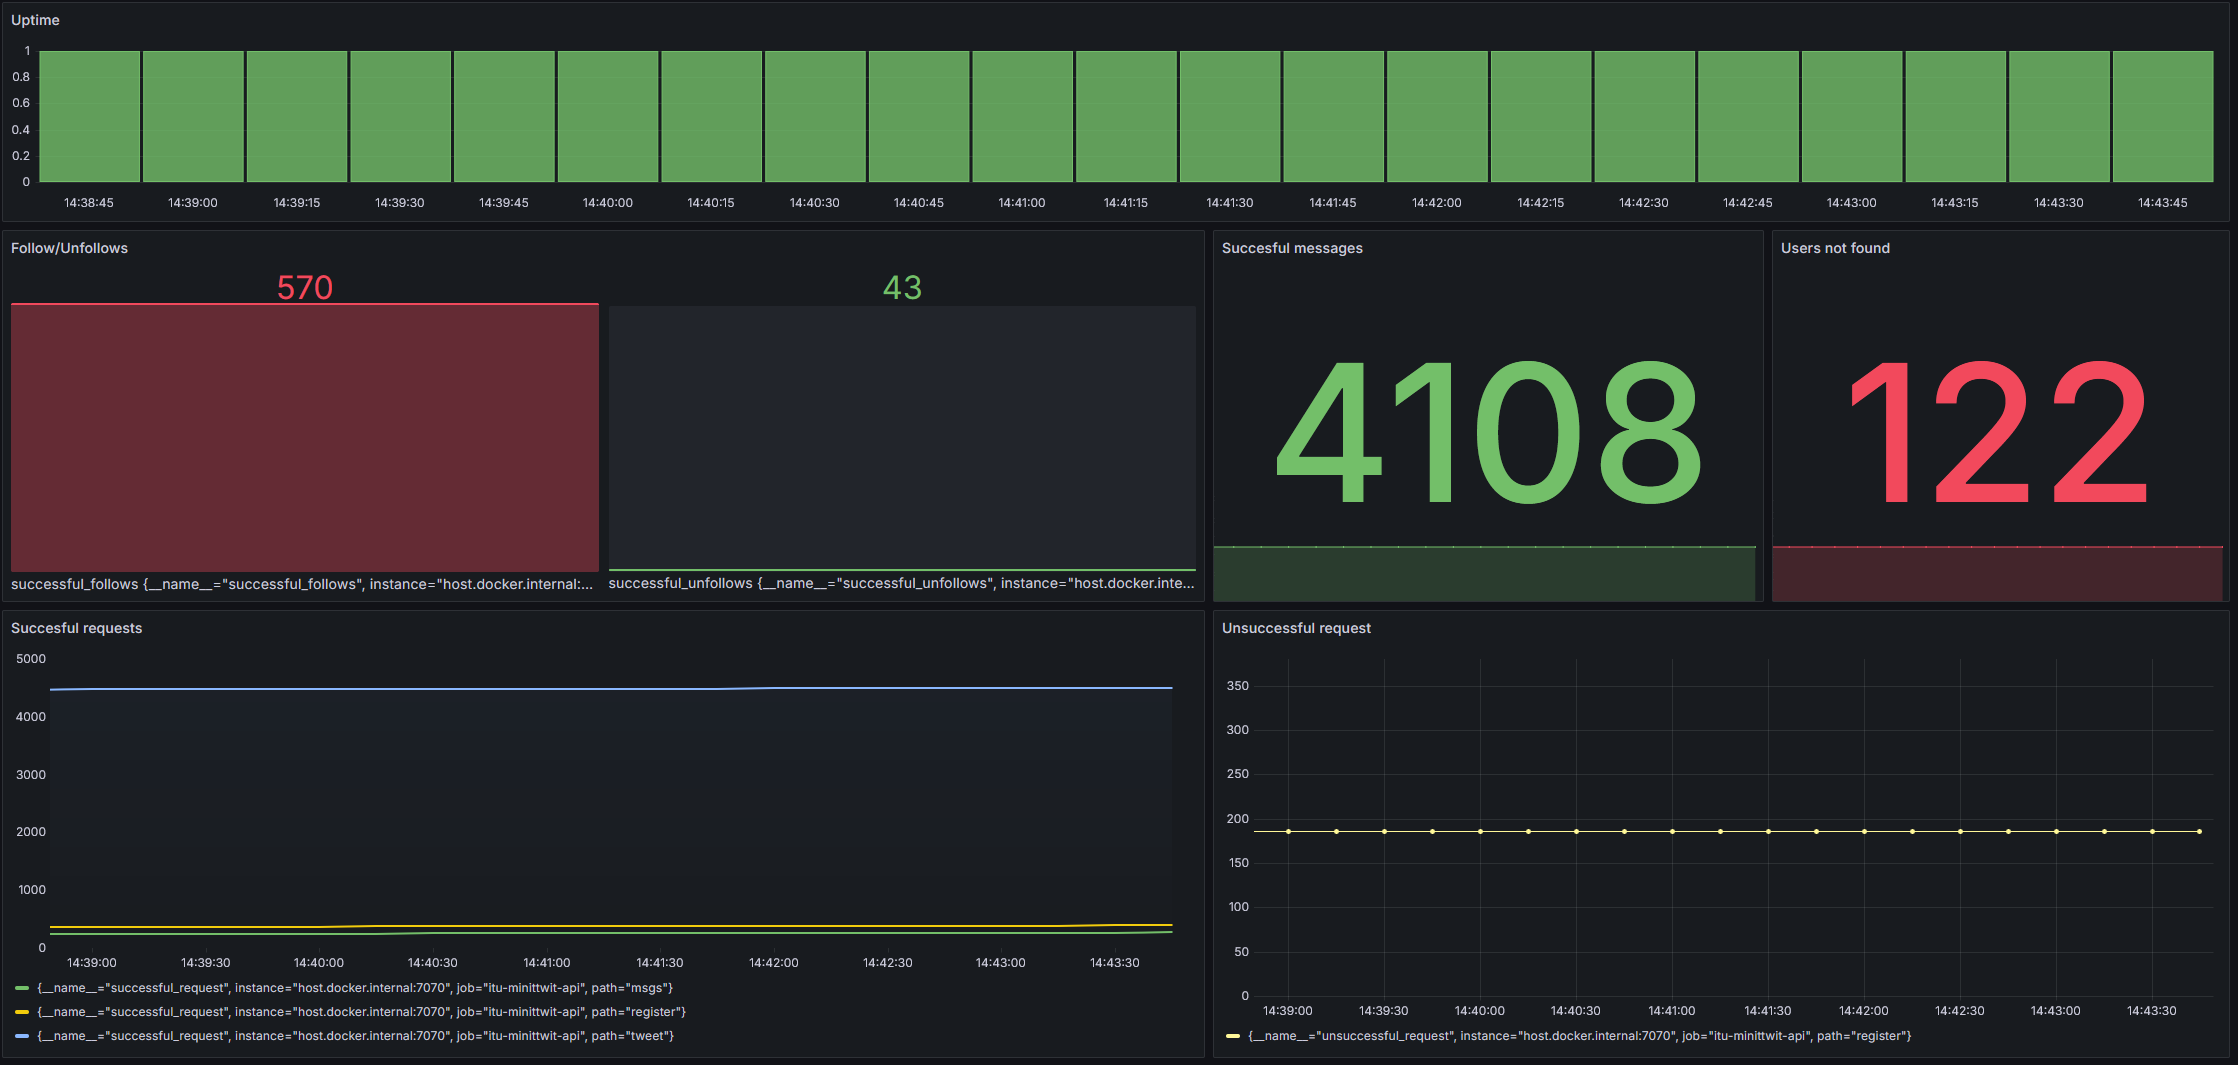
\includegraphics[width=1.0\linewidth]{Images/Grafana_dashboard.png}
    \caption{Screenshot of the Grafana dashboard showing API monitoring metrics}
    \label{fig:dashboard}
\end{figure}

\subsection{Logging}
\label{sec:logging}
For getting the right logs out of our Go application, we used a package called Logrus, which gave us full control over what we wanted to log. By setting the logging level (currently WarnLevel) and using function-level flags we avoided unnecessary verbosity. Since the application handles considerable traffic we deliberately avoided logging every event. Most functions only log when they exceed a 2-second execution threshold to help us focus on performance bottlenecks. We’re also mindful of not logging any sensitive information such as user credentials, tokens or personal data, to ensure compliance with security best practices. However, we don’t yet have a formal log rotation or retention strategy in place, which is something we aim to address as the system scales.\\\\ 

To aggregate logs, we use the ELK Stack. Filebeat collects logs from the Docker containers, and sends these on to Logstash where they are parsed and enriched. Then they are sent to Elasticsearch, which indexes them for efficient querying. Finally, we use Kibana to visualize and analyze the logs through dashboards and search interfaces. This centralized log aggregation gives us access to real-time insight into our distributed application.
%MAX
%What do you log in your systems and how do you aggregate logs?
%make a diagram of the logging stack!

\begin{figure} [!htb]
    \centering
    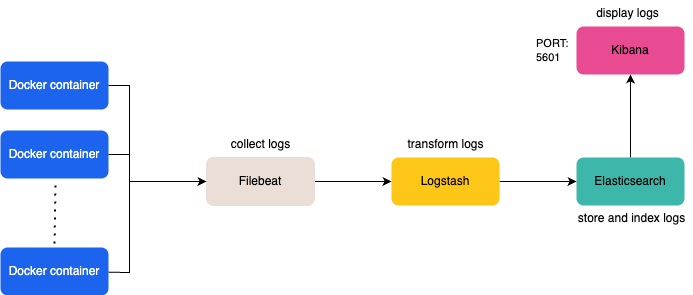
\includegraphics[width=1.0\linewidth]{Images/ELK_diagram.drawio.png}
    \caption{ELK stack used for logging}
    \label{fig:dashboard}
\end{figure}


\subsection{Security Assessment}
%gwen
%Brief results of the security assessment and brief description of how did you harden the security of your system based on the analysis.
Our security assessment revealed threats across various parts of our system. Assets at risk are listed below, along with risk scenarios and how to mitigate them:    
\begin{itemize}
    \item \textbf{Web Application} - An attacker performs SQL injection to extract sensitive user data. This is already mitigated by using ORM methods. A further step would be to automate back-ups of the database.
    
    \item \textbf{Database} - An attacker scraps Github for exposed ports, holding our database for ransom. Again, we should back up the database regularly. Configure firewalls for all droplets and update Docker Compose files.
     
    \item \textbf{API} - An attacker overwhelms the network, causing it to go down. We could avoid this by using Distributed Denial-of-Service (DDOS) protection tools which detect artificial traffic.

    \item \textbf{Github Repository} - Attacker hacks member account and steals Github secrets, exposing all other assets. In general, vulnerable passwords should be strengthened and two-factor authentication (2FA) set up.
    
    \item \textbf{Server} - An intruder gains remote access to the server via SSH, compromising the service. This is partially mitigated as we use GitHub secrets and avoid accidental exposure, however we should ensure all members have 2FA.
    
    \item \textbf{Logs} - If important events (internal or attack) are not logged properly they cannot be traced or followed up. We do already log a lot of errors however there is room for optimisation.

    \item \textbf{Monitoring} - Suspicious activity occurs however the team is not notified resulting in long response times. Ideally, our Grafana dashboard is populated with crucial metrics, e.g. number of requests per sec, and Grafana alerts are activated.

    \item \textbf{Data in Transit} - Internal communications are intercepted by malicious actors, exposing sensitive information. A Transport Layer Security (TLS) is needed to authenticate our servers and encrypt data in transit. 

    \item \textbf{Source Code} - Dependencies get outdated; updates may be incompatible and affect functionality of app. These bugs can be exploited by attackers. We could use tools such as Dependabot to keep our systems up-to-date.

\end{itemize}

The following risk matrix reflects which threats are most important to focus on. Due to time constraints the exposed ports have been addressed using a Docker Compose Linter, and . Ideally, we would also integrate Dependabot, optimise monitoring metrics, use TLS, configure firewalls and automate back-ups of our database as soon as possible.

\begin{figure} [!htb]
    \centering
    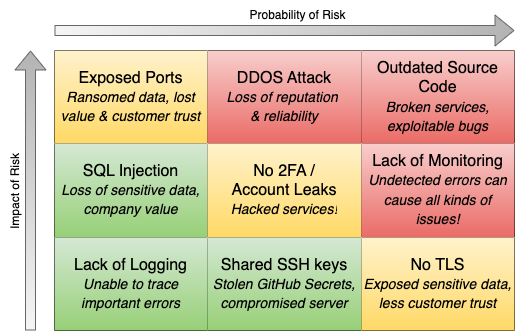
\includegraphics[width=0.7\linewidth]{Images/riskmatrix.png}
    \caption{A risk matrix which takes into account current state of system and mitigations (if any).}
    \label{fig:Seq}
\end{figure}


\subsection{Scaling and Upgrade Strategies}
%Applied strategy for scaling.
%iulia
%A complete description of the failover strategy using hot and standby server and keepalived and update strategy using green blue deployment and the floating ips

\subsubsection{High Availability via Hot-Standby Setup}

To enhance the availability and resilience of our application, we implemented a \textbf{hot-standby server setup} instead of using a container orchestration system like Docker Swarm. In this architecture:
\begin{itemize}
  \item Only one droplet is active at a time, handling all traffic.
  \item A second droplet is in standby mode, kept in sync and ready to take over instantly if the active one fails.
  \item A DigitalOcean floating IP is used to route traffic to the active server and is automatically reassigned during failover.
\end{itemize}

\subsubsection*{Implementation Steps}
We followed these steps to implement the hot-standby architecture:
\begin{itemize}
  \item Created a snapshot of the initial (active) droplet and used it to spawn the standby server.
  \item Assigned a floating IP to the active droplet.
 \item Installed and configured Keepalived on both droplets:
    \begin{itemize}
      \item \texttt{check-api.sh} monitors the health of the application.
      \item \texttt{master.sh} reassigns the floating IP upon failure detection.
      \item \texttt{keepalived.conf} and \texttt{keepalived.service} manage and start the Keepalived daemon.
    \end{itemize}
  \item Added necessary firewall rules and database access permissions on DigitalOcean.
\end{itemize}

\subsubsection*{Why We Chose Hot-Standby over Docker Swarm}
\begin{itemize}
  \item \textbf{Simplicity}: Swarm introduces added complexity and overhead in managing a cluster, which was not justified for our relatively simple application architecture.
  \item \textbf{Predictable failover behavior}: With hot-standby, only one server is live at a time, making debugging and maintenance easier.
  \item \textbf{More control over failover}: The Keepalived setup gives us full control over the logic that triggers failover.
\end{itemize}

\noindent While our hot-standby setup improves availability, it does not horizontally scale the API, meaning only one server handles traffic at a time. However, we opted for vertical scaling by upsizing both droplets and the database to better handle increased load, which we found sufficient for our current scope. If the system was under higher demand, we could have implemented horizontal scaling by running multiple active API replicas behind a load balancer or using a Docker Swarm cluster with service replicas and built-in load distribution.

\subsubsection{Blue-Green Deployment Strategy}

To handle zero-downtime updates and safe rollbacks, we implemented a Blue-Green Deployment Strategy, building on the infrastructure we already had for scaling. 

\noindent We assigned a second floating IP to the standby (passive) droplet. This enabled our CI/CD pipeline to:
\begin{enumerate}
  \item Deploy the new version of the application to the passive server (Blue).
  \item Swap the floating IPs using the DigitalOcean API after a successful deployment, making Blue the new active server (Green).
  \item Redeploy to the now-passive (previously active) server to bring both environments in sync.
\end{enumerate}

\noindent This strategy ensures that:
\begin{itemize}
  \item Deployments are atomic and safe: if the Blue deployment fails, Green remains untouched and continues serving traffic.
  \item Traffic is only routed to stable, verified servers, avoiding mid-deploy errors.
  \item Rollbacks are simple: just reverse the IP swap.
\end{itemize}

\subsubsection*{Why We Chose Blue-Green over Rolling Updates}
\begin{itemize}
  \item \textbf{Minimal complexity}: Our infrastructure is not container-orchestrated, so rolling updates would be harder to coordinate reliably.
  \item \textbf{Clear separation} between active and staging environments.
  \item \textbf{Natural fit with hot-standby}: Using floating IPs made Blue-Green deployment easy to implement with our existing failover setup.
\end{itemize}

